\documentclass[margin=0px]{article}

\usepackage{listings}
\usepackage[utf8]{inputenc}
\usepackage{graphicx}
\usepackage{float}
\usepackage[a4paper, margin=1in]{geometry}
\usepackage{subcaption}
\usepackage{amsthm}
\usepackage{amssymb}
\usepackage{amsmath}
\usepackage{color}

\renewcommand{\figurename}{ábra}
\newenvironment{tetel}[1]{\paragraph{#1 \\}}{}
\newcommand{\R}{\mathbb{R}}

% A dokument itt kezdődik

\title{Záróvizsga tételsor \\ \large 16. Számítógépes hálózatok és Internet eszközök}
\date{}
\author{Dobreff András}

\begin{document}
	\maketitle
	
	\begin{tetel}{Számítógépes hálózatok és Internet eszközök}
			Fizikai réteg, adatkapcsolati réteg, hálózati réteg, szállítói réteg – feladatok, módszerek, protokollok
	\end{tetel}
	
	\section{Hálózatok modelljei}
		\begin{description}
			\item[TCP/IP modell]  \hfill \\
				\textbf{T}ransmission \textbf{C}ontrol \textbf{P}rotocol/\textbf{I}nternet \textbf{P}rotocol. Röviden TCP/IP. A TCP/IP modell 1982-ben lett az amerikai hadászati célú számítógépes hálózatok standardja. 1985-től népszerűsítették kereskedelmi használatra.
				
				4 Réteget különböztet meg:
				\begin{enumerate}
					\item Kapcsolati réteg
					\item Hálózati réteg
					\item Szállítói réteg
					\item Alkalmazási réteg
				\end{enumerate}
			\item[OSI modell]  \hfill \\
				\textbf{O}pen \textbf{S}ystem \textbf{I}nterconnection Reference Model. Röviden OSI referencia modell. Standard koncepcionális modellt definiál kommunikációs hálózatok belső funkcionalitásához.
				
				7 Réteget különböztet meg:
				\begin{enumerate}
					\item Fizikai réteg
					\item Adatkapcsolati réteg
					\item Hálózati réteg
					\item Szállítási réteg
					\item Munkamenet réteg
					\item Megjelenítési réteg
					\item Alkalmazási réteg
				\end{enumerate}
		\end{description}
	\section{Fizikai réteg}
		\begin{description}
			\item[Definíció] \hfill \\
				A fizikai réteg feladata a bitek továbbítása a kommunikációs csatornán keresztül. Azaz a korrekt bit átvitel biztosítása, a kapcsolat kezelése és az átvitelhez szükséges idő és egyéb részletek tisztázása. \\
				Tehát a tervezési szempontok az interfész mechanikai, elektromos és eljárási kérdéseire, illetve az átviteli közegre vonatkoznak.
			\item[Adatátvitel] \hfill
				\begin{description}
					\item[Vezetékes] \hfill \\
						Adatátvitel vezeték esetén valamilyen fizikai jellemző változtatásával lehetséges (pl.: feszültség, áramerősség). Ezt egy $g(t)$ periodikus függvénnyel jellemezhetjük.
						\begin{align*}
							g(t) = \frac{1}{2}c+ \sum\limits_{n=1}^\infty a_nsin(2\pi n f t) + \sum\limits_{n=1}^\infty b_ncos(2\pi n f t) 
						\end{align*}					
						ahol $f=\frac{1}{T}$ az alapfrekvencia, $a_n$ és $b_n$ pedig az $n$-edik harmonikus szinuszos illetve koszinuszos amplitúdók
					\item[Vezetékes nélküli] \hfill \\	
						Vezeték nélküli adatátvitelre sok helyen használnak elektormágneses hullámokat. A hullámoknak van frekvenciája és hullámhossza.
						\begin{itemize}
							\item Frekvencia: 
								A hullám másodpercenkénti rezgésszáma. Jele: $f$, mértékegysége: Hz (Hertz)
							\item Hullámhossz: két egymást követő hullámcsúcs (v. hullámvölgy) közötti távolság. Jele: $\lambda$
						\end{itemize}
						\begin{align*}
							 \lambda f = c
						\end{align*}
						ahol $c$ a fénysebesség, azaz az elektromágneses hullámok terjedési sebessége vákuumban.
						\begin{figure}[H]
							\centering
							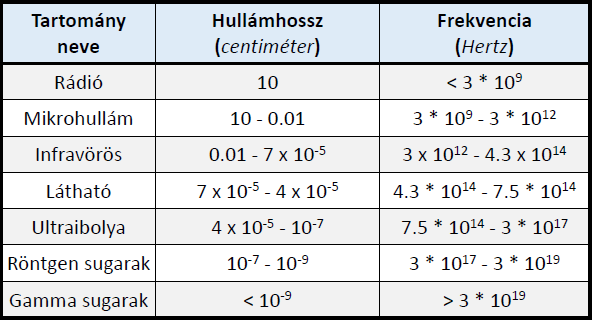
\includegraphics[width=0.6\textwidth]{img/elektromagneses.png}
							\caption{Elektromágneses spektrum}
						\end{figure}
					\item[Szimbólumok] \hfill \\
						Bitek helyett szimbólumokat küldünk át. (Pl. 4 szimbólum: A - 00, B - 01, C - 10, D - 11)\\
						Baud: szimbólum/másodperc \\
						Adatráta: bit/másodperc
					\item[Szinkronizáció] \hfill \\
						Kérdés: Mikor kell szignálokat mérni, illetve mikor kezdődik egy szimbólum? Ehhez szinkronizáció kell a felek között.
						\begin{itemize}
							\item Explicit órajel \\
								Párhuzamos átviteli csatornák használata, szinkronizált adatok, rövid átvitel esetén alkalmas.
							\item Kritikus időpontok \\
								Szinkronizáljunk például egy szimbólum vagy blokk kezdetén, a kritikus időpontokon kívül szabadon futnak az órák, feltesszük, hogy az órák rövid ideig szinkronban futnak.
							\item Szimbólum kódok \\
								Önütemező jel–külön órajel szinkronizáció nélkül dekódolható jel, a szignál tartalmazza a szinkronizáláshoz szükséges információt.
						\end{itemize}
						\begin{figure}[H]
							\centering
							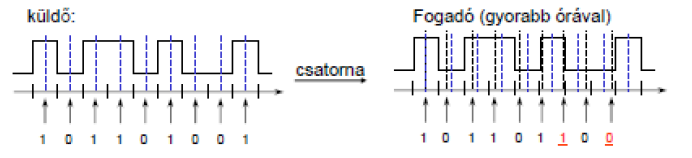
\includegraphics[width=0.6\textwidth]{img/szinkronizacio.png}
							\caption{Szinkronizáció szükségessége}
						\end{figure}
				\end{description}
			\item[Átviteli közegek] \hfill \\
				\begin{description}
					\item[Vezetékes] \hfill
						\begin{itemize}
							\item mágneses adathordozók \\
							sávszélesség jó, késleltetés nagy
							\item sodort érpár \\
							Főként távbeszélőrendszerekben használatos; dupla rézhuzal; analóg és digitális jelátvitel
							\item Koaxális kábel\\
							Nagyobb sebesség és távolság érhető el, mint a sodorttal; analóg és
							digitális jelátvitel
							\item Fényvezető szálak\\
							Fényforrás, átviteli közeg és detektor; fényimpulzus 1-es bit, nincs
							fényimpulzus 0-s bit
						\end{itemize}
					\item[Vezetékes nélküli] \hfill
					\begin{itemize}
					\item Rádiófrekvenciás átvitel \\
					egyszerűen előállíthatóak; nagy távolság; kültéri és beltéri alkalmazhatóság; frekvenciafüggő terjedési jellemzők
					\item Mikrohullámú átvitel\\
					egyenes vonal mentén terjed; elhalkulás problémája; nem drága
					\item Infravörös és milliméteres hullámú átvitel \\
					kistávolságú átvitel esetén; szilárd tárgyakon nem hatol át
					\item Látható fényhullámú átvitel\\ 
					lézerforrás + fényérzékelő; nagy sávszélesség, olcsó, nem engedélyköteles; időjárás erősen befolyásolhatja
					\end{itemize}
				\end{description}
			\item[Jelátvitel] \hfill
				\begin{itemize}
					\item Alapsáv \\
						A digitális jel direkt árammá vagy feszültséggé alakul. A jel minden frekvencián átvitelre kerül. Átviteli korlátok
						\begin{figure}[H]
							\centering
							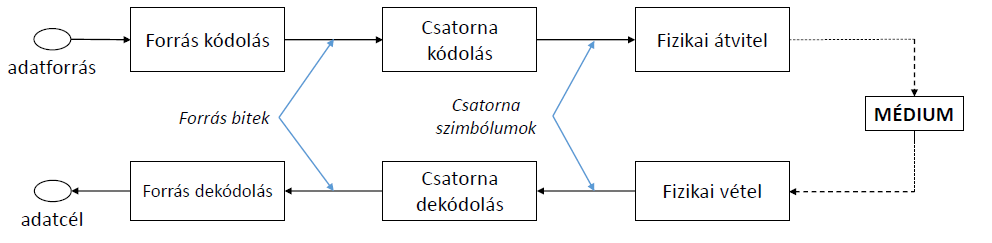
\includegraphics[width=0.8\textwidth]{img/alapsav.png}
							\caption{Digitális alapsávú átvitel struktúrája}
						\end{figure}
					\item Szélessáv \\
						Széles frekvencia tartományban történik az átvitel. A jel modulálására az alábbi lehetőségeket használhatjuk.
						\begin{figure}[H]
							\centering
							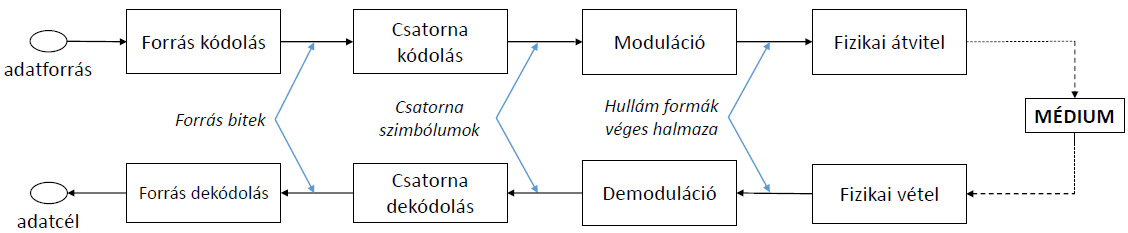
\includegraphics[width=0.8\textwidth]{img/szelessav.png}
							\caption{Digitális szélessávú átvitel struktúrája}
						\end{figure}
						
						Modulációk:\\
						Egy szinuszos rezgés ábrázolása $T$ periódus idejű függvényre $g(t)=Asin(2\pi f t + \varphi)$ , ahol $A$ az amplitúdó, $f = \frac{1}{T}$ a frekvencia és $\varphi $ a fáziseltolás
						\begin{itemize}
							\item Amplitúdó moduláció \\
								Az $s(t)$ szignált a szinusz görbe amplitúdójaként kódoljuk, azaz:
								\begin{align*}
									f_A(t) = s(t) \cdot sin(2\pi f t + \varphi)
								\end{align*}
								Analóg szignál: amplitúdó moduláció\\
								Digitális szignál: amplitúdó keying(szignál erőssége egy diszkrét halmaz értékeinek megfelelően változik)
								\begin{figure}[H]
									\centering
									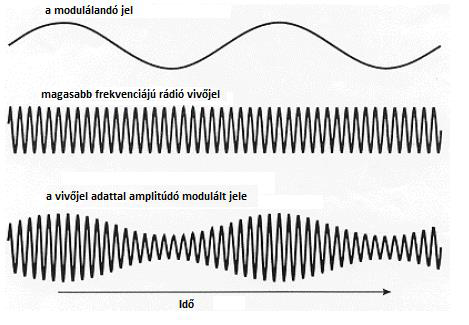
\includegraphics[width=0.5\textwidth]{img/amplitudo_mod.png}
									\caption{Amplitúdó moduláció}
								\end{figure}
								\begin{figure}[H]
									\centering
									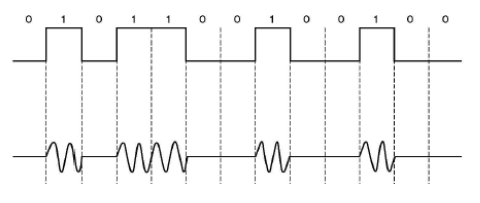
\includegraphics[width=0.5\textwidth]{img/amplitudo_key.png}
									\caption{Amplitúdó keying}
								\end{figure}
							\item Frekvencia moduláció \\
								Az $s(t)$ szignált a szinusz görbe frekvenciájában kódoljuk, azaz:
								\begin{align*}
									f_F(t) = a \cdot sin(2\pi s(t) t + \varphi)
								\end{align*}
								Analóg szignál: frekvencia moduláció\\
								Digitális szignál: frekvencia-eltolás keying(például egy diszkrét halmaz szimbólumaihoz különböző frekvenciák hozzárendelésével)
								\begin{figure}[H]
									\centering
									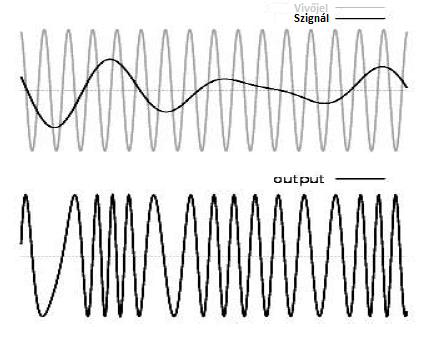
\includegraphics[width=0.5\textwidth]{img/frekvencia_mod.png}
									\caption{Frekvencia moduláció}
								\end{figure}
								\begin{figure}[H]
									\centering
									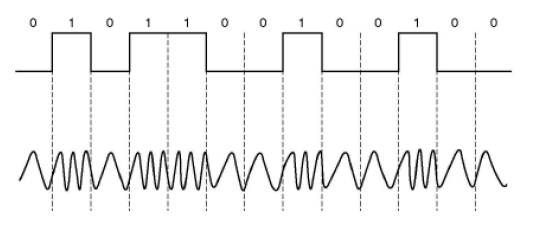
\includegraphics[width=0.5\textwidth]{img/frekvencia_key.png}
									\caption{Frekvencia keying}	
								\end{figure}
							\item Fázis moduláció \\
								Az $s(t)$ szignált a szinusz görbe fázisában kódoljuk, azaz:
								\begin{align*}
								f_P(t) = a \cdot sin(2\pi f t + s(t))
								\end{align*}
								Analóg szignál: fázis moduláció (nem igazán használják)\\
								Digitális szignál: fázis-eltolás keying ( például egy diszkrét halmaz szimbólumaihoz különböző fázisok hozzárendelésével)
								\begin{figure}[H]
									\centering
									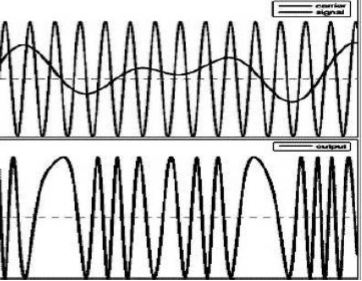
\includegraphics[width=0.5\textwidth]{img/fazis_mod.png}
									\caption{Fázis moduláció}
								\end{figure}
								\begin{figure}[H]
									\centering
									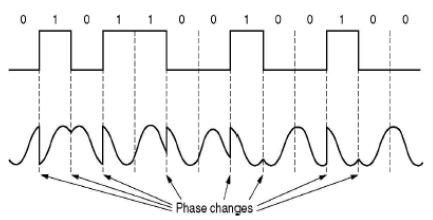
\includegraphics[width=0.5\textwidth]{img/fazis_key.png}
									\caption{Fázis-eltolás keying}	
								\end{figure}
						\end{itemize}
						
						Digitális és analóg jelek összehasonlítása: \\
						Digitális átvitel: Diszkrét szignálok véges halmazát
						használja (például feszültség vagy áramerősség
						értékek).\\
						Analóg átvitel: Szignálok folytonos halmazát használja
						(például feszültség vagy áramerősség a vezetékben) \\
						Digitális esetében lehetőség van a vételpontosság helyreállítására illetve az eredeti jel helyreállítására, míg az analógnál a fellépő hibák önmagukat erősíthetik.
				\end{itemize}
		\end{description}
	\section{Adatkapcsolati réteg}
		\begin{description}
			\item[Definíció] \hfill \\
				Az adatkapcsolati réteg feladata jól definiált szolgálati interfész biztosítása a hálózati rétegnek, melynek három fázisa van:
				\begin{itemize}
					\item nyugtázatlan összeköttetés alapú szolgálat 
					\item nyugtázott összeköttetés nélküli szolgálat 
					\item nyugtázott összeköttetés alapú szolgálat 
				\end{itemize}
				Továbbá az átviteli hibák kezelése és az adatforgalom szabályozása (elárasztás elkerülése).
			\item[Keretképzés] \hfill \\
				A fizikai réteg nem garantál hibamentességet, az adatkapcsolati réteg feladata a hibajelzés illetve a szükség szerint javítás. Erre megoldás: keretekre tördelése a bitfolyamnak, és ellenőrző összegek számítása. A keretezés nem egyszerű feladat, mivel megbízható időzítésre nem nagyon van lehetőség. Négy lehetséges módszer:
				\begin{enumerate}
					\item Karakterszámlálás \\
						A keretben lévő karakterek számát a keret fejlécében adjuk meg. Így a vevő adatkapcsolati rétege tudni fogja a keret végét. Probléma: nagyon érzékeny a hibára a módszer.
						\begin{figure}[H]
							\centering
							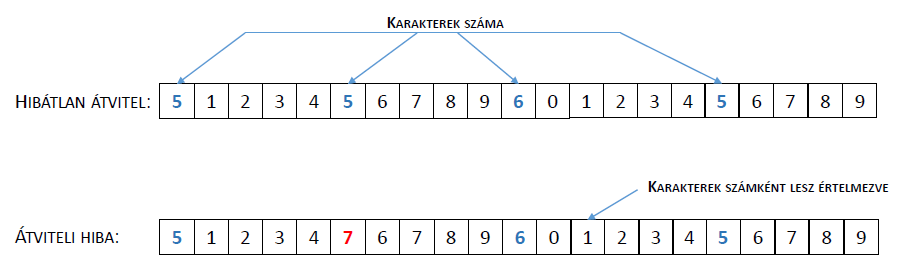
\includegraphics[width=0.7\textwidth]{img/karakterszamlalas.png}
							\caption{Karakterszámlálás}	
						\end{figure}
					\item Kezdő és végkarakterek karakterbeszúrással \\
						Különleges bájtokat helyezünk el a keret elejének és végének jelzésére, aminek a neve jelző bájt(flagbyte). Az adatfolyamban szereplő speciális bájtokhoz ESC bájtot használnak.
						\begin{figure}[H]
							\centering
							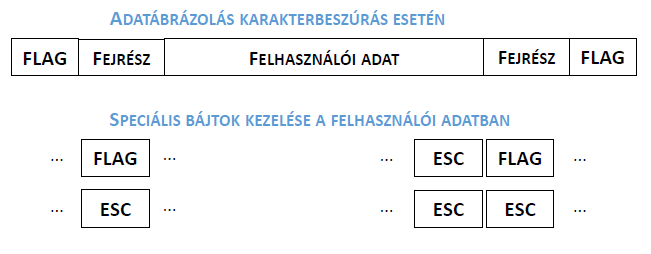
\includegraphics[width=0.6\textwidth]{img/karakterbeszuras.png}
							\caption{Kezdő és végkarakterek karakterbeszúrással}	
						\end{figure}
					\item Kezdő és végjelek bitbeszúrása \\
						Minden keret egy speciális bitmintával kezdődik (flagbájt, 01111110) és minden egymást követő 5 hosszú folytonos 1-es bit sorozat után beszúr egy 0-át.
						\begin{figure}[H]
							\centering
							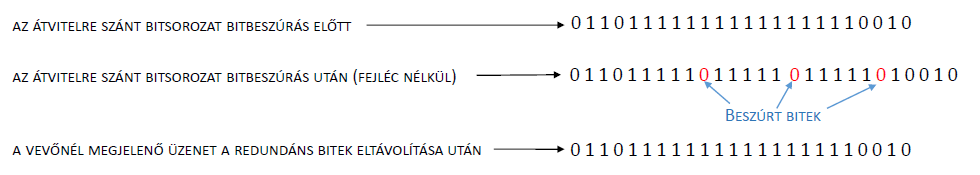
\includegraphics[width=0.9\textwidth]{img/bitbeszuras.png}
							\caption{Kezdő és végjelek bitbeszúrásal}	
						\end{figure}
					\item Fizikai rétegbeli kódolás-sértés \\
						Olyan hálózatokban használható, ahol a fizikai rétegbeli kódolás redundanciát tartalmaz.
				\end{enumerate}
			\item[Hibakezelés] \hfill \\
				Hibakezelés szempontjából a következő két esetet kell vizsgálnunk. A keretek megérkeztek-e a célállomás hálózati rétegéhez, illetve helyes sorrendben érkeztek-e meg. Ehhez valamilyen visszacsatolás szükséges a vevő és az adó között. (például nyugták). Időkorlátokat vezetünk be az egyes lépésekhez. Hiba estén a csomagot újraküldjük. Többszörös vétel lehet, amin segíthet a sorszámok használata. Az adatkapcsolati réteg feladata a hibakezelés szempontjából, hogy az időzítőket és  számlálókat úgy kezelje, hogy biztosítani tudja a keretek pontosan egyszeri (nem több és nem kevesebb) megérkezését a célállomás hálózati rétegéhez.
				
				Bithibák:
				\begin{itemize}
					\item egyszerű bithiba \\
						Az adategység 1 bitje nulláról egyre avagy egyről nullára változik.
						\begin{figure}[H]
							\centering
							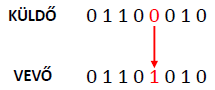
\includegraphics[width=0.2\textwidth]{img/egyszeru_bithiba.png}
							\caption{Egyszerű bithiba}	
						\end{figure}
					\item csoportos bithiba \\
						Egy olyan folytonos szimbólum sorozatot, amelynek az első és utolsó szimbóluma hibás, és nem létezik ezen két szimbólummal határolt részsorozatban olyan $m$ hosszú részsorozat, amelyet helyesen fogadtunk, $m$ hosszú csoportos bithibának nevezünk.
				\end{itemize}
				
				Hiba jelzés és javítás:\\
				Kétféle hibakezelési stratégia létezik. Ezek a hibajelző (redundáns információ mellékelése) és hibajavító kódok (adatok közé iktatott redundancia).
				[Megbízható csatornákon a hibajelzés olcsóbb. (csomagot inkább újraküldjük). A kevésbé megbízható csatornákon a hibajavításos módszer célszerűbb]
				\begin{itemize}
					\item Hamming-távolság, Hamming-korlát \\
						Küldendő keret $m$ bitet tartalmaz. Redundáns bitek száma $r$. Tehát az elküldött keret: $n = m+r$ bit.
						
						Hamming-távolság: \\
						Az olyan bitpozíciók számát, amelyeken a két kódszóban különböző bitek állnak, a két kódszó Hamming távolságának nevezzük. Jelölés: $d(x,y)$\\
						Legyen $S$ az egyenlő hosszú bitszavak halmaza. $S$ Hamming-távolsága:
						\begin{align*}
						d(S) := \min_{x,y, \in S \ \land \ x \neq y} d(x,y)
						\end{align*}
						
						d(S) = 1 esetén: \\
						Nincs hibafelismerés, ugyanis megengedett kódszóból 1 bit megváltoztatásával megengedett kódszó áll elő.
						\begin{figure}[H]
							\centering
							
\includegraphics[width=0.4\textwidth]{img/hamming1.png}
							\caption{Kód Hamming-távolsága = 1}	
						\end{figure}
						d(S) = 2 esetén: \\
						Ha az $x$ kódszóhoz létezik olyan $v$ nem megengedett kódszó, amelyre $d(u,x)=1$, akkor hiba történt. Ha $x$ és $y$ megengedett kódszavak (távolságuk minimális = 2), akkor a következő összefüggésnek teljesülnie kell:
						\begin{align*}
							2 = d(x,y) \leq d(x,v)+d(v,y)
						\end{align*}
						Azaz egy bithiba felismerhető, de nem javítható.
						\begin{figure}[H]
							\centering
							
\includegraphics[width=0.4\textwidth]{img/hamming2.png}
							\caption{Kód Hamming-távolsága = 2}	
						\end{figure}
						
						d(S) = 3 esetén: \\
						Ekkor minden $u$, melyre $d(x,u)=1$ és $d(u,y) > 1$ nem megengedett. Ekkor három lehetőség áll fent:
						\begin{itemize}
							\item x került átvitelre és 1 bit hibával érkezett
							\item y került átvitelre és 2 bit hibával érkezett
							\item valami más került átvitelre és legalább 2 bit hibával érkezett
						\end{itemize}
						De valószínűbb, hogy $x$ került átvitelre, tehát ez egy 1 bit hiba javító, 2 bit hiba felismerő kód.
						\begin{figure}[H]
							\centering
							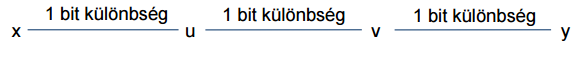
\includegraphics[width=0.4\textwidth]{img/hamming3.png}
							\caption{Kód Hamming-távolsága = 3}	
						\end{figure}
						
						Hamming-korlát: \\
						$ C \subseteq \{0,1\}^n$ és $d(C) = k$. Ekkor a kódszavak $\frac{k-1}{2}$ sugarú környezeteiben található bitszavak egymással diszjunkt halmazainak uniója legfeljebb az $n$-hosszú bitszavak halmazát adhatja ki. Vagyis formálisan:
						\begin{align*}
						|C|\sum_{i=0}^{\lfloor\frac{k-1}{2}\rfloor}\dbinom{n}{i} \leq 2^n
						\end{align*}
							
						\begin{itemize}
							\item Hibafelismerés: \\
								$d$ bit hiba felismeréséhez a keretek halmazában legalább $d+1$ Hamming távolság szükséges.
							
							\item Hibajavítás: \\
								$d$ bit hiba javításához a megengedett keretek halmazában legalább $2d+1$ Hamming távolság szükséges.
							
							\item Kód rátája: \\
								$R_S = \frac{log_2|S|}{n}$ a kód rátája ($S \subseteq \{0,1\}^n$) - hatékonyságot karakterizálja
							
							\item Kód távolsága: \\
								$\delta_S = \frac{d(S)}{n}$ a kód távolsága  ($S \subseteq \{0,1\}^n$) - hibakezelést karakterizálja
						\end{itemize}
						A jó kódnak a rátája és a távolsága is nagy.
					\item Paritásbit \\
						A paritásbit olyan bit, melyet a kódszóban lévő egyesek száma alapján választunk.
						\begin{itemize}
							\item Odd Parity - ha az egyesek száma páratlan, akkor 0 befűzése; egyébként 1-es befűzése
							\item Even Parity - ha az egyesek száma páros, akkor 0 befűzése; egyébként 1-es befűzése
						\end{itemize}
						Egy paritást használó módszer az ún. Hamming módszer:\\
						A kódszó bitjeit számozzuk meg (1-gyel kezdődően). A 2 hatványú pozíciókon az ellenőrző bitek kapnak helyet, a maradék helyekre az üzenet bitjei kerülnek. Mindegyik ellenőrző bit a bitek egy csoportjának (beleértve önmagát is) a paritását állítja be párosra (vagy páratlanra).\\
						A csoportok a következőképp alakulnak:
						\begin{itemize}
							\item 1. bit: Minden első egyhosszú bitsorozat az első bittől kezdve (tehát: 1,3,5,7,...)
							\item 2. bit: Minden első kéthosszú bitsorozat a második bittől kezdve (tehát: 2-3,6-7,10-11)
							\item 4. bit: Minden első négyhosszú bitsorozat a negyedik bittől kezdve (tehát: 4-7,12-15)
							\item stb.
						\end{itemize}
						\begin{figure}[H]
							\centering
							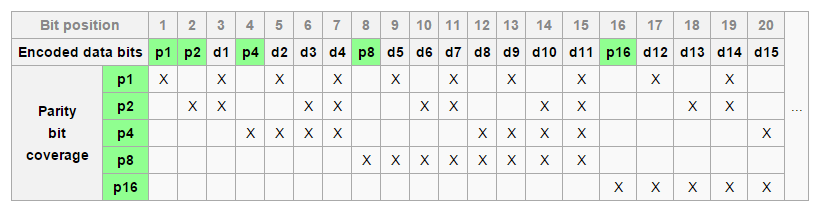
\includegraphics[width=0.8\textwidth]{img/paritasbit.png}
							\caption{Paritásbitek csoportjai}	
						\end{figure}
						Példa:\\
						Legyen az átküldendő üzenet: 1000101 \\
						Ekkor a kódszó a következőképp alakul: \\
							{\color[rgb]{1,0,0}$\heartsuit\heartsuit$}1{\color[rgb]{1,0,0}$\heartsuit$}000{\color[rgb]{1,0,0}$\heartsuit$}101\\
							A 8. bit a 8-11  bitsorozat paritását állítja be párosra:\\
							{\color[rgb]{1,0,0}$\heartsuit\heartsuit$}1{\color[rgb]{1,0,0}$\heartsuit$}000{\color[rgb]{0,0,1}0101}\\
							A 4. bit a 4-7  bitsorozat paritását állítja be párosra:\\
							{\color[rgb]{1,0,0}$\heartsuit\heartsuit$}1{\color[rgb]{0,0,1}0000}0101\\
							A 2. bit a 2-3, 6-7, 10-11 bitsorozat paritását állítja be párosra:\\
							{\color[rgb]{1,0,0}$\heartsuit$}{\color[rgb]{0,0,1}01}00{\color[rgb]{0,0,1}00}01{\color[rgb]{0,0,1}01}\\
							Az 1. bit az 1,3,5,7,9,11 bitsorozat paritását állítja be párosra: \\
							{\color[rgb]{0,0,1}1}0{\color[rgb]{0,0,1}1}0{\color[rgb]{0,0,1}0}0{\color[rgb]{0,0,1}0}0{\color[rgb]{0,0,1}1}0{\color[rgb]{0,0,1}1}\\
							
							Tehát a elküldendő bitsorozat:
							{\color[rgb]{1,0,0}10}1{\color[rgb]{1,0,0}0}000{\color[rgb]{1,0,0}0}101\\
				
					\item CRC - Polinom-kód, azaz ciklikus redundancia \\
						A bitsorozatokat egy $\mathbb{Z}_2$ feletti polinom ($M(x)$) együtthatóinak tekintjük. Definiálunk egy $G(x)$ $r$ fokú generátorpolinomot, melyet a vevő és küldő egyaránt ismer.
						\begin{enumerate}
							\item Fűzzünk $r$ darab 0 bitet a keret alacsony helyi értékű végéhez. Azaz vegyük az $x^rM(x)$ polinomot (ez már $m+r$ fokú)
							\item Osszuk el $x^rM(x)$-et $G(x)$-szel (mod 2).
							\item A maradékot (mely mindig r vagy kevesebb bitet tartalmaz) vonjuk ki $x^rM(x)$-ből (mod 2). Így az eredeti keret végére egy r hosszú ellenőrző összeg kerül. Legyen ez a polinom $T(x)$.
							\item A vevő egy $T(x)+E(x)$-nek megfelelő polinomot kap (ahol $E(x)$ a hiba polinom). Ezt elosztva a generátorpolinommal egy $R(x)$ polinomot kapunk. Ha ez a polinom nem nulla, akkor hiba történt.
						\end{enumerate}
						A $G(x)$ többszöröseinek megfelelő bithibákat nem ismerjük fel.
				\end{itemize}
			\item[Protokollok] \hfill
				\begin{description}
					\item[Elemi adatkapcsolati protokollok] \hfill 
						 \begin{itemize}
						 	\item Korlátozás nélküli szimplex protokoll\\
							 	Környezet:
							 	\begin{itemize}
							 		\item Adó, vevő: mindig kész.
							 		\item Nincs feldolgozási idő
							 		\item Végtelen puffer
							 		\item Nincs keret rontás, vesztés
							 	\end{itemize}
							 	
							 	Protokoll:
							 	\begin{itemize}
							 		\item Nincs sorszám/nyugta
							 		\item Küldő végtelen ciklusban küldi kifele a kereteket folyamatosan
							 		\item A vevő kezdetben várakozik az első keret megérkezésére, keret érkezésekor a hardver puffer tartalmát változóba teszi és az adatrészt továbbküldi a hálózati rétegnek.
							 	\end{itemize}
						 	\item Szimplex megáll és vár protokoll 	\\
							 	Környezet:
							 	\begin{itemize}
							 		\item Adó, vevő hálózati rétegei: mindig kész.
							 		\item A vevőnek $\delta t$ időre van szüksége a bejövő keret feldolgozására.
							 		\item Nincs pufferelés és sorban állás sem
							 		\item Nincs keret rontás, vesztés
							 	\end{itemize}
							 	
							 	Protokoll:
							 	\begin{itemize}
							 		\item Nincs sorszám/nyugta
							 		\item Küldő egyesével küld, következőt csak a nyugtát követően.
							 		\item A vevő kezdetben várakozik az első keret megérkezésére, keret érkezésekor a hardver puffer tartalmát változóba teszi és az adatrészt továbbküldi a hálózati rétegnek, végül nyugtázza a keretet.
							 	\end{itemize}
						 	\item Szimplex protokoll zajos csatornához\\
							 	Környezet:
							 	\begin{itemize}
							 		\item Adó, vevő hálózati rétegei: mindig kész.
							 		\item A vevőnek $\delta t$ időre van szüksége a bejövő keret feldolgozására.
							 		\item Nincs pufferelés és sorban állás sem
							 		\item Keret sérülhet, elveszhet
							 	\end{itemize}
							 	
							 	Protokoll:
							 	\begin{itemize}
							 		\item Nincs sorszám/nyugta
							 		\item Küldő egyesével küld, addig nem küld újat, míg határidőn belül nyugtát nem kap. Határidő után újraküldi a keretet.
							 		\item A vevő kezdetben várakozik az első keret megérkezésére, keret érkezésekor a hardver puffer tartalmát változóba teszi, leellenőrzi a kontroll összeget:
							 		\begin{itemize}
							 			\item Nincs hiba: az adatrészt továbbküldi a hálózati rétegnek, végül nyugtázza a keretet.
							 			\item Van hiba: eldobja a keretet és nem nyugtáz
							 		\end{itemize}
							 	\end{itemize}
						 \end{itemize}
					\item[Csúszóablakos protokoll] \hfill \\
						Egy adott időpontban egyszerre több keret is átviteli állapotban lehet. A fogadó $n$ keretnek megfelelő méretű puffert allokál. A küldőnek legfeljebb $n$, azaz ablak méretnyi, nyugtázatlan keretet küldése engedélyezett. A keret sorozatbeli pozíciója adja a keret címkéjét. (sorozatszám).
						A fogadónak a hibás, illetve a nem megengedett sorozatszámmal érkező kereteket el kell dobnia. A küldő nyilvántartja a küldhető sorozatszámok halmazát (adási ablak). A fogadó nyilvántartja a fogadható sorozatszámok halmazát (vételi ablak). Az adási ablak minden küldéssel szűkül, illetve nő egy nyugta érkezésével.
						
						Mi van ha egy hosszú folyam közepén történik egy keret hiba?
						\begin{enumerate}
							\item "visszalépés N-nel" stratégia\\
								Az összes hibás keret utáni keretet eldobja és nyugtát sem küld róluk. Mikor az adónak lejár az időzítője, akkor újraküldi az összes nyugtázatlan keretet, kezdve a sérült vagy elveszett kerettel. Hátrány: Nagy sávszélességet pazarolhat el, ha nagy a hibaarány.
							\item "szelektív ismétlés" stratégia \\
								A hibás kereteket eldobja, de a jó kereteket a hibás után puffereli. Mikor az adónak lejár az időzítője, akkor a legrégebbi nyugtázatlan keretet küldi el újra. Hátrány: Nagy memória igény nagy vételi ablak esetén.
						\end{enumerate}
						
					\item[Példák adatkapcsolati protokollokra] \hfill
						\begin{itemize}
							\item HDLC - High-level Data Link Control \\
								A HDLC protokoll 3 bites csúszó-ablak protokollt alkalmaz  a sorszámozáshoz. 
								Három típusú keretet használ:
								\begin{itemize}
									\item információs
									\item felügyelő
									\begin{itemize}
										\item nyugtakeret (RECIEVE READY)
										\item negatív nyugta keret (REJECT)
										\item vételre nem kész (RECIEVE NOT READY) - nyugtáz minden keretet a következőig
										\item szelektív elutasítás (SELECTIVE REJECT) - egy gy adott keret újraküldésére szólít fel 
									\end{itemize}
									\item Számozatlan
								\end{itemize}
								
								Általános keretfelépítése:
								\begin{itemize}
									\item FLAG bájt a keret határok jelzésére
									\item \textit{cím} mező - több vonallal rendelkező terminálok esetén van jelentősége
									\item \textit{vezérlés} mező - sorszámozás, nyugtázás és egyéb feladatok ellátására
									\item \textit{adat} mező - tetszőleges hosszú adat lehet
									\item \textit{ellenőrző összeg} mező - CRC kontrollösszeg  (CRC-CCITT generátor polinom felhasználásával)
								\end{itemize}
								\begin{figure}[H]
									\centering
									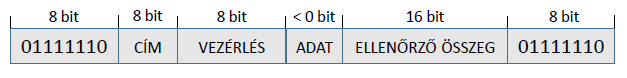
\includegraphics[width=0.8\textwidth]{img/hdlc_keret.png}
									\caption{HDLC keret felépítése}	
								\end{figure}
							\item PPP - Point-to Point Protocol \\
								A PPP protokoll három dolgot biztosít:
								\begin{itemize}
									\item  Keretezési módszert (egyértelmű kerethatárok)
									\item Kapcsolatvezérlő protokollt (a vonalak felélesztésére, tesztelésére, az opció egyeztetésére és a vonalak elengedésére.)
									\item Olyan módot a hálózati réteg-opciók megbeszélésére, amely független az alkalmazott hálózati réteg-protokolltól.
								\end{itemize} 
								Bájt alapú keretszerkezet használ (azaz a legkisebb adategység a bájt).
								Vezérlő mező alapértéke a számozatlan keretet jelzi. Protokoll mezőben protokoll kód lehet az LCP, NCP, IP, IPX, AppleTalkvagy más protokollhoz.
								\begin{figure}[H]
									\centering
									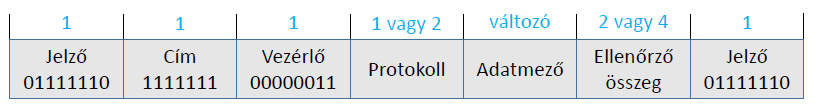
\includegraphics[width=0.8\textwidth]{img/ppp_keret.png}
									\caption{PPP keret felépítése}	
								\end{figure}
						\end{itemize}
					\item[MAC - Media Access Control] \hfill \\
						Eddigi tárgyalásaink során pont-pont összeköttetést feltételeztünk. Most az adatszóró csatornát használó hálózatok tárgykörével foglalkozunk majd. A csatorna kiosztás történhet statikus vagy dinamikus módon.
						
						Statikus esetben vagy Frekvenciaosztásos nyalábolást vagy időosztásos nyalábolást használnak. Frekvenciaosztásos esetben a sávszélességet osztják $N$ részre, és mindegyik felhasználó egy sávot kap. Időosztásos esetben az időegységet osztják $N$ részre és ezeket adják a felhasználóknak. Mind a két módszer löketszerű forgalom esetén nem tud hatékony lenni.
						
						A továbbiakban a dinamikus csatorna kiosztási módszereket vizsgáljuk.
						\begin{itemize}
							\item Verseny protokollok \\
								N független állomás van, amelyeken egy program vagy egy felhasználó továbbítandó kereteket generál. Ha egy állomás generált egy keretet, akkor blokkolt állapotban marad mindaddig, amíg a keretet sikeresen nem továbbította. Egyetlen csatorna van, melyen mindenféle kommunikáció zajlik. Minden állomás tud adatot küldeni és fogadni ezen a csatornán. Ha két keret egy időben kerül átvitelre, akkor átlapolódnak, és az eredményül kapott jel értelmezhetetlenné válik. Ezt nevezzük ütközésnek. Ez minden állomás számára felismerhető. Az ütközésben érintett kereteket később újra kell küldeni. (Ezen a hibán kívül egyéb hiba nem történhet.)
								
								Kétféle időmodellt különböztetünk meg:
								\begin{enumerate}
									\item Folytonos – Mindegyik állomás tetszőleges időpontban megkezdheti a küldésre kész keretének sugárzását.
									\item Diszkrét – Az időt diszkrét résekre osztjuk. Keret továbbítás csak időrés elején lehetséges. Az időrés lehet üres, sikeres vagy ütközéses
								\end{enumerate}
								
								Az egyes állomások vagy rendelkeznek vivőjel érzékeléssel vagy nem. Ha nem, akkor az állomások nem tudják megvizsgálni a közös csatorna állapotát, ezért egyszerűen elkezdenek küldeni, ha van rá lehetőségük. Ha igen, akkor az állomások meg tudják vizsgálni a közös csatorna állapotát a küldés előtt. A csatorna lehet: foglalt vagy szabad. Ha a foglalt a csatorna, akkor nem próbálják használni az állomások, amíg fel nem szabadul
								
								\begin{itemize}
									\item Egyszerű ALOHA \\
										A felhasználó akkor vihet át adatot, amikor csak szeretne. Ütközés esetén véletlen ideig várakozik az állomás, majd újra próbálkozik.
										
										Keret idő–egy szabványos, fix hosszúságú keret átviteléhez szükséges idő
										
										Egy keret akkor nem szenved ütközést, ha elküldésének első pillanatától kezdve egy keretideig nem próbálkozik más állomás keretküldéssel.
										
										\begin{figure}[H]
											\centering
											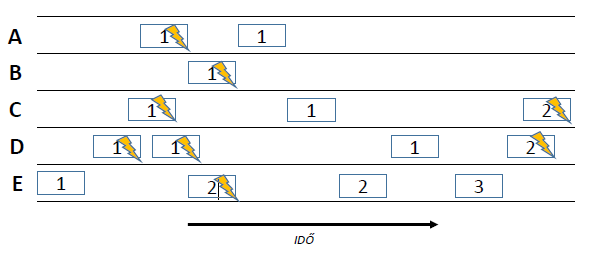
\includegraphics[width=0.6\textwidth]{img/egyszeru_aloha.png}
											\caption{Egyszerű ALOHA keret ütközések}	
										\end{figure}
									\item Réselt ALOHA \\
										Az idő diszkrét, keretidőhöz igazodó időszeletek-re osztásával az ALOHA rendszer kapacitása megduplázható. A csatorna terhelésének kis növekedése is drasztikusan csökkentheti a médium teljesítményét.
									\item 1-prezisztens CSMA \\
										Vivőjel érzékelés van, azaz minden állomás belehallgathat a csatornába. Folytonos időmodellt használ a protokoll. 

										Algoritmus:
										\begin{enumerate}	
											\item Keret leadása előtt belehallgat a csatornába:
											\begin{enumerate}
												\item Ha foglalt, akkor addig vár, amíg fel nem szabadul. Szabad csatorna esetén azonnal küld. (perzisztens)
												\item Ha szabad, akkor küld.
											\end{enumerate}
											\item Ha ütközés történik, akkor az állomás véletlen hosszú ideig vár, majd újrakezdi a keret leadását.
										 \end{enumerate}
									\item Nem-prezisztens CSMA \\
										Vivőjel érzékelés van, azaz minden állomás belehallgathat a csatornába. Folytonos időmodellt használ a protokoll. Mohóságot kerüli, azaz nem küld azonnal, ha foglalt.
										
										Algoritmus:
										\begin{enumerate}	
											\item Keret leadása előtt belehallgat a csatornába:
											\begin{enumerate}
												\item Ha foglalt, akkor véletlen ideig vár (nem figyeli a forgalmat), majd kezdi előröl a küldési algoritmust. (nem-perzisztens)
												\item Ha szabad, akkor küld.
											\end{enumerate}
											\item Ha ütközés történik, akkor az állomás véletlen hosszú ideig vár, majd újrakezdi a keret leadását.
										\end{enumerate}
									\item p-prezisztens CSMA \\
										Vivőjel érzékelés van, azaz minden állomás belehallgathat a csatornába. Diszkrét időmodellt használ a protokoll. 
										
										Algoritmus:
										\begin{enumerate}	
											\item Adás kész állapotban az állomás belehallgat a csatornába:
											\begin{enumerate}
												\item Ha foglalt, akkor vár a következő időrésig, majd megismétli az algoritmust.
												\item Ha szabad, akkor $p$ valószínűséggel küld, illetve $1-p$ valószínűséggel visszalép a szándékától a következő időrésig. Várakozás esetén a következő időrésben megismétli az algoritmust. Ez addig folytatódik, amíg el nem küldi a keretet, vagy amíg egy másik állomás el nem kezd küldeni, mert ilyenkor úgy viselkedik, mintha ütközés történt volna.
											\end{enumerate}
											\item Ha ütközés történik, akkor az állomás véletlen hosszú ideig vár, majd újrakezdi a keret leadását.
										\end{enumerate}
									\item CSMA/CD \\
										Ütközés érzékelés esetén meg lehessen szakítani az adást. Minden állomás küldés közben megfigyeli a csatornát, ha ütközést tapasztalna, akkor megszakítja az adást, és véletlen ideig várakozik, majd újra elkezdi leadni a keretét
								\end{itemize}
								\begin{figure}[H]
									\centering
									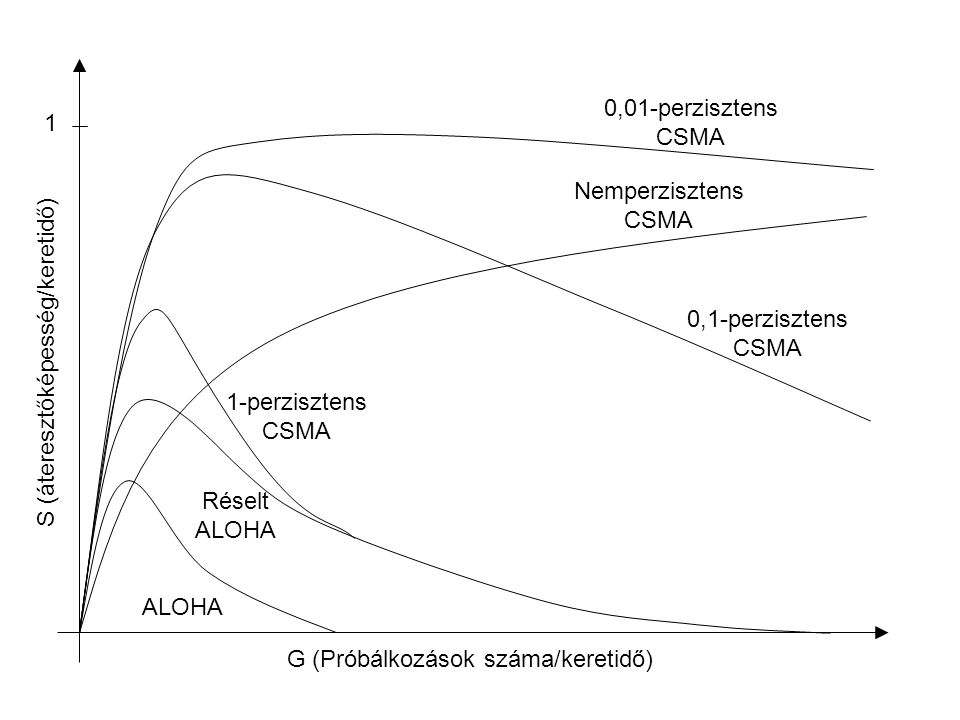
\includegraphics[width=0.7\textwidth]{img/aloha_csma.jpg}
									\caption{ALOHA és CSMA protokollok összehasonlítása}	
								\end{figure}
							\item Verseny mentes protokollok \\
								Motiváció: Az ütközések hátrányosan hatnak a rendszer teljesítményére, és a CSMA/CD nem mindenhol alkalmazható.

								N állomás van. Az állomások 0-ától N-ig egyértelműen sorszámozva vannak. Réselt időmodellt feltételezünk.
								\begin{itemize}
									\item Egy helyfoglalásos protokoll \\
										Ha az i-edikállomás küldeni szeretne, akkor a i-edikversengési időrésben egy 1-es bit elküldésével jelezheti. Így a versengési időszak végére minden állomás ismeri a küldőket. A küldés a sorszámok szerinti sorrendben történik meg.
									\item Bináris visszaszámlálás protokoll \\
										Minden állomás azonos hosszú bináris azonosítóval rendelkezik. A forgalmazni kívánó állomás elkezdi a bináris címét bitenként elküldeni a legnagyobb helyi értékű bittel kezdve. Az azonos pozíciójú bitek logikai VAGY kapcsolatba lépnek ütközés esetén. Ha az állomás nullát küld, de egyet hall vissza, akkor feladja a küldési szándékát, mert van nála nagyobb azonosítóval rendelkező küldő.
								\end{itemize}
							\item Korlátozott verseny protokollok \\
							Olyan protokoll, amely kis terhelés esetén versenyhelyzetes technikát használ a kis késleltetés érdekében, illetve nagy terhelés mellett ütközésmentes technikát alkalmaz a csatorna jó kihasználása érdekében.
								\begin{itemize}
									\item Adaptív fabejárás \\
									Minden állomást egy egyértelmű, bináris ID reprezentál. Az ID-k egy (bináris) fa leveleinek felelnek meg. Az időrések a fa egyes csomópontjaihoz vannak rendelve Minden időrésben megvizsgáljuk az adott csomópont alatti részfát. A fa egy $u$ csomópontjánál 3 esetet
									különböztethetünk meg:
									\begin{itemize}
										\item Egy állomás sem küld az $u$ részfában.
										\item Pontosan egy állomás küld az $u$ részfában.
										\item Több állomás küld az $u$ részfában. Ezt nevezzük kollíziónak.
									\end{itemize}
									Kollízió esetén hajtsuk végre az ellenőrzést $u$ bal, és jobb oldali gyerekére egyaránt.
									
									Ezzel a módszerrel könnyen megállapítható, hogy melyik állomás küldhet az adott időszeletben.
									\begin{figure}[H]
										\centering
										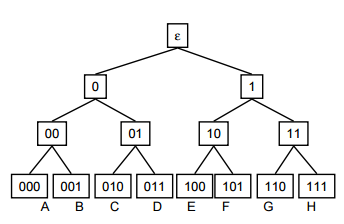
\includegraphics[width=0.5\textwidth]{img/adaptivfa.png}
										\caption{Adaptív fabejárás protokoll bináris fája}	
									\end{figure}
								\end{itemize}							
						\end{itemize}
				\end{description}
		\end{description}
	\section{Hálózati réteg}
		\begin{description}
			\item[Definíció] \hfill \\
				A hálózati réteg fő feladata a csomagok továbbítása a forrás és a cél között. Ez a legalacsonyabb olyan réteg, amely két végpont közötti átvitellel foglalkozik. Ismernie kell a kommunikációs alhálózat topológiáját. Ügyelni kell, hogy ne terheljen túl se bizonyos kommunikációs útvonalakat, se bizonyos routereket úgy, hogy mások tétlen maradnak.
				
				A szállítási réteg felé nyújtott szolgálatok:
				\begin{itemize}
					\item Függetlenek az alhálózatok kialakításától
					\item Eltakarják a jelen lévő alhálózatok számát, típusát és topológiáját
					\item A szállítási réteg számára rendelkezésre bocsájtott hálózati címek egységes számozási rendszert kell alkotnak
				\end{itemize}
			\item[Forgalom irányítás típusai] \hfill
				\begin{itemize}
					\item Hierarchikus forgalomirányítás\\
						Routhereket tartományokra osztjuk. A saját tartományát az összes router ismeri, de a többi belső szerkezetéről nincs tudomása. Nagy hálózatok esetén többszintű hierarchia lehet szükséges. 
					\item Adatszóró forgalomirányítás\\
						egy csomag mindenhová történő egyidejű küldése.
					\item Többküldéses forgalomirányítás\\ 
						Egy csomag meghatározott csoporthoz történő egyidejű küldése.
						
				\end{itemize}

			\item[Forgalom irányító algoritmusok] \hfill \\
				A hálózati réteg szoftverének azon része, amely azért a döntésért felelős, hogy a bejövő csomag melyik kimeneti vonalon kerüljön továbbításra. A folyamat két lépésre bontható:
				\begin{enumerate} 
					\item Forgalomirányító táblázatok feltöltése és karbantartása.
					\item Továbbítás
				\end{enumerate}
				
				A forgalomirányító algoritmusok osztályai:
				\begin{enumerate}
					\item Adaptív algoritmusok
					\begin{enumerate}
						\item távolság alapú
						\item kapcsolat alapú
					\end{enumerate}
						A topológia és rendszerint a forgalom is befolyásolhatja a döntést.
					\item Nem-adaptív algoritmusok \\
						Offline meghatározás, betöltés a router-ekbe induláskor
				\end{enumerate}
			
				\begin{description}
					\item[Dijkstra algoritmus] \hfill \\
						A Dijkstra algoritmus egy statikus algoritmus, melynek célja két csomópont közötti legrövidebb út meghatározása.

						Minden csomópontot felcímkézünk a kezdőpontból az addig megtalált legrövidebb út hosszával. Az algoritmus működése során a címkék változhatnak az utak megtalálásával. Két fajta címkét különböztetünk meg: ideiglenes és állandó. Kezdetben minden címke ideiglenes. A legrövidebb út megtalálásakor a címke állandó címkévé válik, és továbbá nem változik.
					\item[Elárasztás algoritmus] \hfill \\
						Elárasztás algoritmusa egy statikus algoritmus.
						
						Minden bejövő csomagot minden kimenő vonalon továbbítunk kivéve azon, amin érkezett. Így azonban nagyon sok duplikátum keletkezne. Ezért
						\begin{itemize}
							\item Ugrásszámlálót vezetünk be, melyet minden állomás eggyel csökkent. Ha 0-ra csönnen, eldobják.
							\item Az állomások nyilvántartják a már kiküldött csomagokat. Így egy csomagot nem küldenek ki többször.
						\end{itemize}
					\item[Elosztott Bellman-Ford algoritmus] \hfill \\
						Az Elosztott Bellman-Ford algoritmus adaptív, távolság alapú forgalomirányító algoritmus. Minden csomópont csak a közvetlen szomszédjaival kommunikálhat. Minden állomásnak van saját távolság vektora. Ezt periodikusan elküldi a direkt szomszédoknak. Minden router ismeri a közvetlen szomszédjaihoz a költséget. A kapott távolság vektorok alapján minden csomópont aktualizálja a saját vektorát. 
					\item[Kapcsolatállapot alapú forgalomirányítás] \hfill \\
						A kapcsolatállapot alapú forgalomirányító algoritmusnak a motivációja, hogy a távolság alapú algoritmusok lassan konvergáltak, illetve az eltérő sávszélek figyelembevétele. \\
						A kapcsolatállapot alapú forgalomirányító algoritmus lépései:
						\begin{enumerate}
							\item Szomszédok felkutatása, és hálózati címeik meghatározása
							\item Megmérni a késleltetést vagy költséget minden szomszédhoz
							\item Egy csomag összeállítása a megismert információkból
							\item Csomag elküldése az összes többi router-nek
							\item Kiszámítani a legrövidebb utat az összes többi router-hez.
						\end{enumerate}
				\end{description}
			\item[Hálózat réteg az Interneten] \hfill \\
				A hálózati réteg szintjén az internet autonóm rendszerek összekapcsolt együttesének tekinthető. Nincs igazi szerkezete, de számos főbb gerinchálózata létezik. A gerinchálózatokhoz csatlakoznak a területi illetve regionális hálózatok. A regionális és területi hálózatokhoz csatlakoznak az egyetemeken, vállalatoknál és az internet szolgáltatóknál lévő LAN-ok.
				
				Az internet protokollja, az IP.
				
				Az Interneten a kommunikáció az alábbi módon működik:
				\begin{enumerate}
					\item A szállítási réteg viszi az adatfolyamokat és datagramokra tördeli azokat.
					\item Minden datagram átvitelre kerül az Interneten, esetleg menet közben kisebb egységekre darabolva.
					\item A célgép hálózati rétege összeállítja az eredeti datagramot, majd átadja a szállítási rétegének.
					\item A célgép szállítási rétege beilleszti a datagramot a vételi folyamat bemeneti adatfolyamába.
				\end{enumerate}
				
				Internet Protokoll - IP
					\begin{itemize}
						\item Az IP fejrésze:
							\begin{itemize}
								\item verzió:\\
								IP melyik verzióját használja
								\item IHL: \\
								a fejléc hosszát határozza meg
								\item szolgálat típusa: \\
								szolgálati osztályt jelöl
								\item teljes hossz: \\
								fejléc és adatrész együttes hossza bájtokban
								\item azonosítás: \\
								egy datagram minden darabja ugyanazt az azonosításértéket hordozza.
								\item DF: \\
								"ne darabold" flag a router-eknek
								\item MF: \\
								"több darab" flag minden darabban be kell legyen állítva, kivéve az utolsót.
								\item darabeltolás: \\
								a darab helyét mutatja a datagramon belül.
								\item élettartam: \\
								másodpercenként kellene csökkenteni a mező értékét, minden ugrásnál csökkentik eggyel az értékét
								\item protokoll: \\
								szállítási réteg protokolljának azonosítóját tartalmazza
								\item ellenőrző összeg: \\
								a router-eken belüli rossz memóriaszavak által előállított hibák kezelésére használt ellenőrző összeg a fejrészre, amelyet minden ugrásnál újra kell számolni
								\item forrás cím és cél cím: \\
								IP cím
								\item opciók: \\
								következő verzió bővíthetősége miatt hagyták benne.
							\end{itemize}
							
							\begin{figure}[H]
								\centering
								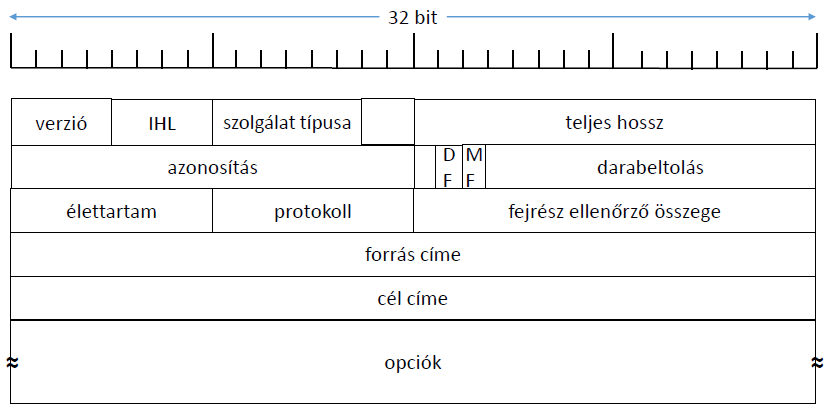
\includegraphics[width=0.8\textwidth]{img/ip_fejresz.png}
								\caption{IPv4 fejléce}
							\end{figure}
							
							\item IP cím \\
								Minden hoszt és minden router az Interneten rendelkezik egy IP-címmel, amely a hálózat számát és a hoszt számát kódolja. 4 bájton ábrázolják az IP-címet. Az IP-t pontokkal elválasztott decimális rendszerben írják. (Például: 192.168.0.1) Van pár speciális cím (ábra \ref{fig:ip_spec_cimek}).
								
								\begin{figure}[H]
									\centering
									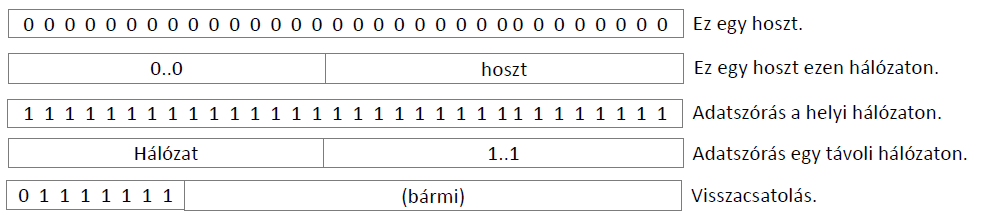
\includegraphics[width=0.8\textwidth]{img/ip_spec_cimek.png}
									\caption{Speciális IP címek}
									\label{fig:ip_spec_cimek}
								\end{figure}
								
								Alhálózatok:\\
								Az azonos hálózatban lévő hosztok ugyanazzal a hálózatszámmal rendelkeznek. Egy hálózat belső felhasználás szempontjából több részre osztódhat, de a külvilág számára egyetlen hálózatként jelenik meg. Azonosításnál az alhálózati maszk ismerete kell a routernek. A forgalomirányító táblázatba a router-eknél (hálózat,0) és (saját hálózat, hoszt) alakú bejegyzések. Ha nincs találat, akkor az alapértelmezett router felé továbbítják a csomagot.\\
								
								IP címek fogyása:\\
								Az IP címek gyorsan fogytak. Megoldás: osztályok nélküli környezetek közötti forgalomirányítás (CIDR). A forgalomirányítás megbonyolódik: Minden bejegyzés egy 32-bites maszkkal egészül ki. Egy bejegyzés innentől egy hármassal jellemezhető: (ip-cím, alhálózati maszk, kimeneti vonal). Új csomag esetén a cél címből kimaszkolják az alhálózati címet, és találat esetén a leghosszabb illeszkedés felé továbbítják.
								
								Másik módszer a NAT, ami gyors javítás az IP címek elfogyásának problémájára. Az internet forgalomhoz minden cégnek egy vagy legalábbis kevés IP-címet adnak, míg vállalaton belül minden számítógéphez egyedi IP-címet használnak a belső forgalomirányításra: \\
								10.0.0.0 – 10.255.255.255 : 16 777 216 egyedi cím\\
								172.16.0.0 – 172.31.255.255 : 1 048 576 egyedi cím\\
								192.168.0.0 – 192.168.255.255 : 65 536 egyedi cím\\
								
								IPv6:\\
								Az IPv4-gyel szemben 16 bájt hosszú címeket használ; 8 darab, egyenként négy-négy hexadecimális számjegyből álló csoportként írjuk le. (Például: 8000:0000:0000:0000:0123:4567:89AB:CDEF) Az IP fejléc egyszerűsödött, amely lehetővé teszi a router-eknek a gyorsabb feldolgozást. A biztonság irányába jelentős lépés történt. 
								
								\begin{figure}[H]
									\centering
									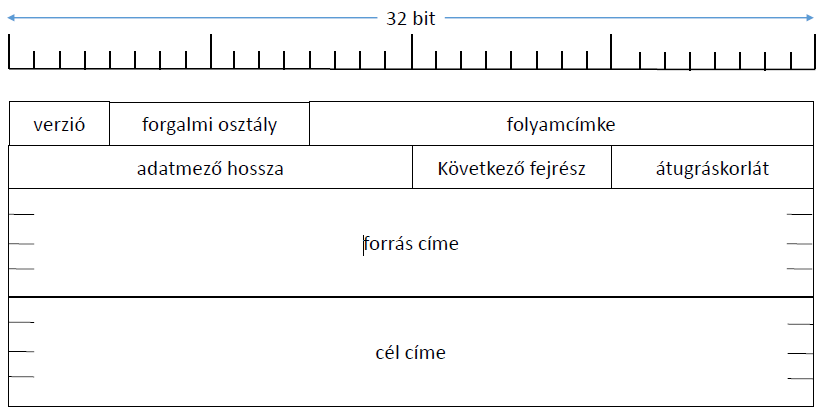
\includegraphics[width=0.8\textwidth]{img/ipv6.png}
									\caption{IPv6 fejléce}
								\end{figure}
								
								
					\end{itemize}
			\item[Protokollok] \hfill
			\begin{itemize}
				\item Internet Control Message Protocol - ICMP \\
					Feladata a váratlan események jelentése. Többféle ICMP-üzenetet definiáltak:
					\begin{itemize}
						\item Elérhetetlen cél
						\item Időtúllépés
						\item Paraméterprobléma
						\item Forráslefojtás
						\item Visszhang kérés
						\item Visszhang válasz
						\item etc.
					\end{itemize}
				\item Address Resolution Protocol - ARP \\
					Feladata az IP cím megfeleltetése egy fizikai címnek. Egy "Kié a 192.60.34.12-es IP-cím?" csomagot küld ki az Ethernet-re adatszórással az alhálózaton. Minden egyes host ellenőrzi,hogy övé-e a kérdéses IP-cím. Ha egyezik az IP a hoszt saját IP-jével, akkor a saját Ethernet címével válaszol.
				\item Reverse Address Resolution Protocol - RARP \\
					Feladatat a fizikai cím megfeleltetése egy IP címnek. Az újonnan indított állomás adatszórással csomagot küld ki az Ethernetre: "A 48-bites Ethernet-címem 14.04.05.18.01.25. Tudja valaki az IP címemet?" Az RARP-szerver pedig válaszol a megfelelő IP címmel, mikor meglátja a kérést.
				\item Open Shortest Path First - OSPF \\
					Az OSPF az AS-eken (Autonomus System) belüli forgalomirányításért felel. A hálózat topológiáját térképezi fel, és érzékeli a változásokat. A topológiát egy súlyozott irányított gráffal reprezentálja, melyben legolcsóbb utakat keres. 
				\item Border Gateway Protocol - BGP \\
					Feladata hogy a politikai szempontok szerepet játsszanak az AS-ek közötti forgalomirányítási döntésekben (Pl. Az IBM-nél kezdődő illetve végződő forgalom ne menjen át a Microsoft-on vagy Csak akkor haladjunk át Albánián, ha nincs más út a célhoz.)\\
					A BGP router szempontjából a világ AS-ekből és a közöttük átmenő vonalakból áll. (Két AS összekötött, ha van köztük a BGP-router-eiket összekötő vonal.)
					Az átmenő forgalom szempontjából 3 féle hálózat van:
					\begin{itemize}
						\item Csonka hálózatok, amelyeknek csak egyetlen összeköttetésük van a BGP gráffal
						\item Többszörösen bekötött hálózatok, amelyeket használhatna az átmenő forgalom, de ezek ezt megtagadják
						\item Tranzit hálózatok, amelyek némi megkötéssel, illetve általában fizetség ellenében, készek kezelni harmadik fél csomagjait
					\end{itemize}
			\end{itemize}
		\end{description}
	\section{Szállítói réteg}
		\begin{description}
			\item[Definíció] \hfill \\
			A szállítási réteg biztosítja, hogy a felhasználók közötti adatátvitel transzparens (átlátszó) legyen. A réteg biztosítja, és ellenőrzi egy adott kapcsolat megbízhatóságát. Az alkalmazási rétegtől kapott adat elejére egy úgynevezett fejlécet csatol, mely jelzi, hogy melyik szállítási rétegbeli protokollal küldik az adatot. Néhány protokoll kapcsolat orientált. Ez azt jelenti, hogy a réteg nyomon követi az adatcsomagokat, és hiba esetén gondoskodik a csomag vagy csomagok újraküldéséről. 
			
			\item[Kapcsolat nélküli és kapcsolatorientált] \hfill \\
				 A kapcsolatorientált protokoll elfedi az alkalmazások előtt az átvitel esetleges hibáit, nem kell törődnünk az elveszett, vagy duplán megérkezett, illetve sérült csomagokkal, és azzal sem, hogy milyen sorrendben érkeztek meg. Viszont ez rontja a teljesítményét.
				 
				 Kapcsolat nélküli esetben nincs szükség az adat keretekre bontására, és nincs  csomagújraküldés.
			\item[Megbízhatóság] \hfill \\
				A megbízhatóság ismérvei:
				\begin{itemize}
					\item Minden csomag megérkezése nyugtázásra kerül.
					\item A nem nyugtázott adatcsomagokat újraküldik.
					\item A fejléchez és a csomaghoz ellenőrzőösszeg van rendelve.
					\item A csomagokat számozza, és a fogadónál sorba rendezésre kerülnek a csomagok a sorszámaik alapján.
					\item Duplikátumokat törli.
				\end{itemize}
			\item[Torlódásfelügyelet] \hfill \\
				Minden hálózaton  korlátos az átviteli sávszélessége. Ha több adatot vezetünk a hálózatba, akkor az torlódáshoz (congestion) vezet, vagy akár a hálózat összeomlásához (congestive collapse). Következmény: Az adatcsomagok nem érkeznek meg.

				Lavina jelenség: \\
				A hálózat túlterhelése csomagok elvesztését okozza, ami csomag újraküldését eredményezi. Az újraküldés tovább növeli a hálózat terhelését így még nagyobb lesz csomagvesztés. Ez még több újraküldött csomagot eredményez. ... \\
				A torlódás felügyelet feladata a lavina jelenség elkerülése.
				
				Követelmények a torlódásfelügyelettel szemben:
				\begin{itemize}
					\item Hatékonyság: \\
						Az átvitel nagy, míg a késés kicsi.
					\item Fairness: \\
						Minden folyamat megközelítőleg azonos részt kap a sávszélességből. (Priorizálás lehetősége fennáll)
				\end{itemize}
				
				A torlódásfelügyelet eszközei:
				\begin{itemize}
					\item Kapacitásnövelés
					\item Erőforrás foglalás és hozzáférés szabályzás
					\item Terhelés csökkentése és szabályzása
				\end{itemize}
				
				Stratégiák:
				\begin{itemize}
					\item Csúszóablak \\
						Adatráta szabályozása ablak segítségével. A fogadó határozza meg az ablak (wnd) méretét. Ha a fogadási puffere tele van, lecsökkenti 0-ra, egyébként \textgreater0-t küld. A küldő nem küld több csomagot, ha az elküldött még nem nyugtázott csomagok száma elérte az ablak méretét. 	
						\begin{figure}[H]
							\centering
							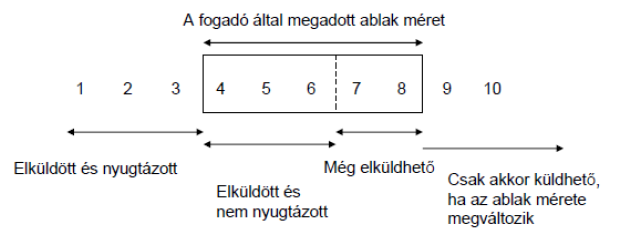
\includegraphics[width=0.6\textwidth]{img/csuszoablak.png}
							\caption{Csúszóablak}
						\end{figure}
					\item Slow-start \\
						A küldőnek nem szabad a fogadó által küldött ablakméretet azonnal kihasználni. Meghatároz egy másik ablakot (cwnd - Congestion Window), melyet ő választ. Ezután végül amiben küld: min\{wnd, cwnd\}. Kezdetben cwnd = MSS (Maximum Segment Size). Minden csomagnál a megkapott nyugta után növeli: cwnd = cwnd + MSS (azaz minden RTT után duplázódik). Ez addig megy, míg a nyugta egyszer kimarad.
					\item TCP-Nagle \\
						Biztosítani kell, hogy a kis csomagok időben egymáshoz közel kerüljenek kiszállításkor, illetve hogy sok adat esetén a nagy csomagok részesüljenek előnyben. \\
						Ehhez: A kis csomagok nem kerülnek kiküldésre, míg nyugták hiányoznak (egy csomag kicsi, ha az adathossz \textless MSS). Ha a korábban küldött csomag nyugtája megérkezik, küldi a következőt.
					\item TCP Tahoe és Reno
						A TCP csúszóablakot és a Slow-start mechanizmusát is használja. Habár a kezdő ráta kicsi, az ablak mérete rohamosan nő. Amikor a cwnd eléri az ssthresh (slow start threshold) értéket átvált torlódás elkerülési állapotba. A TCP Tahoe és Reno torlódás elkerülési algoritmusok. A két algoritmus abban különbözik, hogy hogyan detektálják és kezelik a csomag vesztést. \\
						\underline{TCP Tahoe}: A torlódás detektálására egy időzítőt állít a várt nyugta megérkezésére. 
						\begin{itemize}
							\item Kapcsolatfelvételkor: cwnd = MSS, ssthresh = $2^{16}$
							\item Csomagvesztésnél : Multiplicative decrease \\ 
								cwns = MSS, ssthresh = 	max\{2MSS, $\frac{min\{cwnd, wnd\}}{2}$\}
							\item cwnd $\leq $ ssthresh : Slow-start \\
								cwnd = cwnd + MSS
							\item cwnd \textgreater ssthresh : Additive Increase \\
								cwnd = 	cwnd + MSS$frac{MSS}{cwnd}$
						\end{itemize}
						\underline{TCP Reno}: A torlódás detektálásához időzítőt és gyors újraadást is használ. [Gyors újraadás: ugyanazon csomaghoz 3 nyugta duplikátum érkezik (4 azonos nyugta), akkor újraküldi a csomagot és Slow-start fázisba lép.] \\
						Gyors újraadás után: ssthresh = max\{$\frac{min\{wnd,cwnd\}}{2}$, 2MSS\}, cwnd = sstresh + 3MSS. \\
						Gyors visszaállítás a gyors újraadás után minden további nyugta után növeli a rátát : cwnd = cwnd + MSS.
				\end{itemize}

				Hatékonyság és Fairness: \\
				Az átvitel maximális, ha a terhelés a hálózat kapacitását majdnem eléri. Ha a terhelés tovább nő, túlcsordulnak a pufferek, csomagok vesznek el, újra kell küldeni, drasztikusan nő a válaszidő. Ezt a torlódásnak nevezzük. Ezért a maximális terhelés helyett, ajánlatos a hálózat terhelését a könyök közelében beállítani. Itt a válaszidő csak lassan emelkedik, míg az adatátvitel már a maximum közelében van
				
				Egy jó torlódáselkerülési (angolul congestion avoidance) stratégia a hálózat terhelését a könyök közelében tartja: \textit{hatékonyság}. Emellett fontos, hogy minden résztvevőt egyforma rátával szolgáljunk ki: \textit{fairness}
				
				Jelölje az $i$-edik résztvevő adatrátáját a $t$ időpontban $x_i(t)$.
				Minden résztvevő aktualizálja az adatrátáját a $t+1$-ik fordulóban:
				\begin{align*}
					x_i(t+1) = f_0(t) \quad  ha \ \sum_{i=1}^{n}x_i(t) \leq K \\
					x_i(t+1) = f_1(t) \quad  ha \ \sum_{i=1}^{n}x_i(t) > K
				\end{align*}
				ahol $f_0(x) = a_I + b_Ix$ a növelési, $f_1(x) = a_D + b_Dx$ a csökkentési stratégia.
				
				Speciálsi esetek:
				\begin{itemize}
					\item \textbf{M}ultiplcative \textbf{I}ncrease \textbf{M}ultiplcative \textbf{D}ecrease - MIMD:
					\begin{align*}
						f_0(x) = b_Ix \quad (b_I > 1)\\
						f_1(x) = b_Dx \quad (b_D < 1)
					\end{align*}
					\item \textbf{A}dditive \textbf{I}ncrease \textbf{A}dditive \textbf{D}ecrease - AIAD:
					\begin{align*}
						f_0(x) = a_I+x \quad (a_I > 0)\\
						f_1(x) = a_D+x \quad (a_D < 0)					
					\end{align*}
					\item \textbf{A}dditive \textbf{I}ncrease \textbf{M}ultiplcative \textbf{D}ecrease - AIMD:
					\begin{align*}
						f_0(x) = a_I+x \quad (a_I > 0)\\
						f_1(x) = b_Dx \quad (b_D < 1)
					\end{align*}
				\end{itemize}
				
			\item[Multiplexálás, demultiplexálás] \hfill \\
				Multiplexelés alatt a telekommunikációban azt az eljárást értik, amikor két vagy több csatornát összefognak egy csatornába úgy, hogy az inverz multiplexelés művelettel, vagy demultiplexeléssel, vagy demuxálással elő tudják állítani az eredeti csatornákat. Az eredeti csatornák egy úgynevezett kódolási sémával azonosíthatóak.
			\item[Interakciós modellek] \hfill
				\begin{itemize}
					\item Kétirányú bájtfolyam \\
						Az adatok két egymással ellentétes irányú bájt-sorozatként kerülnek átvitelre. A tartalom nem interpretálódik Az adatcsomagok időbeli viselkedése megváltozhat: átvitel sebessége növekedhet, csökkenhet, más késés, más sorrendben is megérkezhetnek. Megpróbálja az adatcsomagokat időben egymáshoz közel kiszállítani. Megpróbálja az átviteli közeget hatékonyan használni.
					
					\item RPC \\
						A távoli gépen futtatandó eljárás eléréséhez hálózati kommunikációra van szükség, ezt az eljáráshívási mechanizmust az RPC (Remote Procedure Call) fedi el. 
						
						A hívás lépései:
						\begin{enumerate}
							\item A kliensfolyamat lokálisan meghívja a
							klienscsonkot.
							\item Az becsomagolja az eljárás azonosítóját
							és paramétereit, meghívja az OS-t.
							\item Az átküldi az üzenetet a távoli OS-nek.
							\item Az átadja az üzenetet a
							szervercsonknak.
							\item Az kicsomagolja a paramétereket,
							átadja a szervernek.
							\item A szerver lokálisan meghívja az eljárást,
							megkapja a visszatérési értéket.
							\item Ennek visszaküldése a klienshez
							hasonlóan zajlik, fordított irányban.
					\end{enumerate}
					\begin{figure}[H]
						\centering
						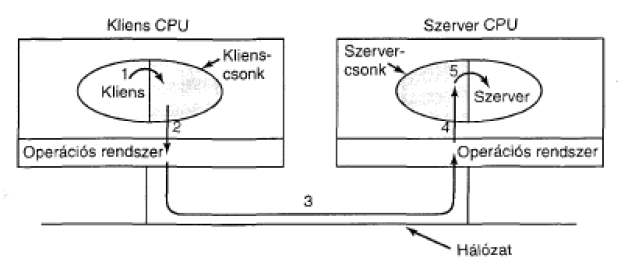
\includegraphics[width=0.6\textwidth]{img/rpc.png}
						\caption{RPC}
					\end{figure}
				\end{itemize}
			\item[Protokollok] \hfill 
				\begin{itemize}
					\item TCP
						\begin{itemize}
							\item Megbízható adatfolyam létrehozása két végpont között
							\item Az alkalmazási réteg adatáramát osztja csomagokra
							\item A másik végpont a csomagok fogadásról nyugtát küld
						\end{itemize}
						A TCP fejléc tartalma:
						\begin{itemize}
							\item küldő port(16 bit)\\
								A küldő folyamatot azonosítja
							\item cél port(16 bit)\\
								A címzett folyamat azonosítója
							\item sorszám(32 bit)\\ 
								Az első adatbájt sorszáma az aktuális szegmensen belül. Ha a SYN jelzőbit értéke 1, akkor ez a sorszám a kezdeti sorszám, azaz az első adatbájt sorszáma a kezdeti sorszám + 1 lesz.
							\item nyugtaszám(32 bit)\\
								Ha az ACK jelzőbit értéke 1, akkor a fogadó által következőnek fogadni 	kívánt sorszámot tartalmazza. Minden kapcsolat felépítés esetén elküldésre kerül.
							\item fejléc hossza (4 bit)\\
								A TCP fejléc hossza 32-bites egységekben.
							\item Ablak(16 bit)\\
								A nyugtázott bájttal kezdődően hány bájtot lehet elküldeni. (A 0 érték is érvényes.)
							\item Ellenőrzőösszeg(16 bit)\\
								Az adat-, fej-, és pszeudofejrész ellenőrzésére.
							 \item Opciók(0-40 bájt)\\
								 A szabványos fejlécen kívüli lehetőségekre tervezték. Legfontosabb ilyen lehetőség az MSS, azaz a legnagyobb szegmens méret megadása. További opciók: MD5-aláírás, TCP-AO, "usertimeout", stb.
							 \item sürgősségi mutató(16 bit) \\
								 A sürgős adat bájtban mért helyét jelzi a jelenlegi bájtsorszámhoz viszonyítva.
							 \item Jelző bitek (6)
								 \begin{enumerate}
							 		\item URG – Sürgős jelzőbit.
							 		\item ACK – nyugta jelzés.
							 		\item PSH – Az jelzi, hogy gyors adattovábbítás kell a felhasználói rétegnek.
							 		\item RST – Kapcsolat egyoldalú bontását jelzi.
							 		\item SYN – Sorszám szinkronizációtjelez.
							 		\item FIN – Adatfolyam végét jelzi.
								 \end{enumerate}		 
							\end{itemize}
							\begin{figure}[H]
								\centering
								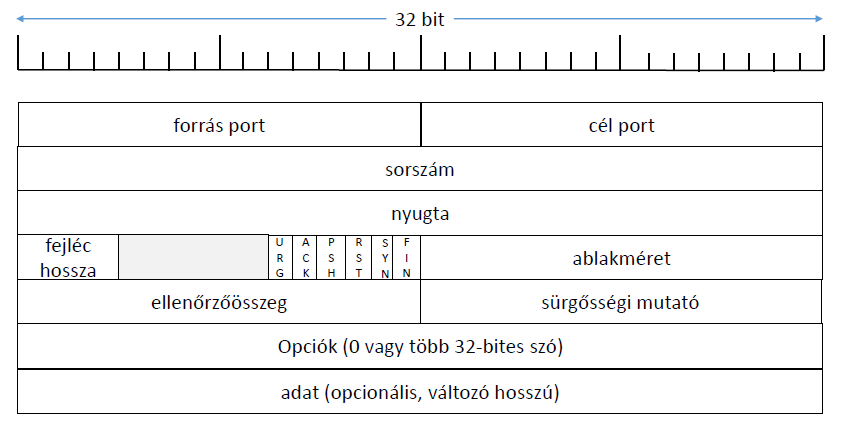
\includegraphics[width=0.8\textwidth]{img/tcp_fejlec.png}
								\caption{TCP Fejléc}
							\end{figure}
							TCP jellemzői:
							\begin{itemize}
								\item Kapcsolatorientált
								\item Megbízható
								\item Kétirányú bájtfolyam
							\end{itemize}
					\item UDP
						\begin{itemize}
							\item Egyszerű, nem megbízható szolgáltatás csomagok küldésére
							\item Az alkalmazási réteg határozza meg a csomag méretét
							\item Az inputot egy datagrammá alakítja	
						\end{itemize}
						Összeköttetés nélküli protokoll. Olyan szegmenseket használ az átvitelhez, amelyek egy 8 bájtos fejrészből, valamint a felhasználói adatokból állnak.\\
						A Fejrész tartalmaz:
						\begin{itemize}
							\item egy forrásportot(2 bájt);
							\item egy célportot(2 bájt);
							\item egy UDP szegmens hossz értéket (2 bájt);
							\item egy UDP ellenőrzőösszeget (2 bájt)		
						\end{itemize}
						Az UDP nem végez forgalomszabályozást, hibakezelést vagy újraküldést egy rossz szegmens fogadása után. Kliens-szerver alkalmazások esetén kifejezetten hasznos lehet az UDP a rövid üzenetek miatt.
				\end{itemize}
		\end{description}
\end{document}